\documentclass[tikz,border=10pt]{standalone}

\usepackage{tikz}
\usetikzlibrary{arrows.meta, positioning}

\begin{document}

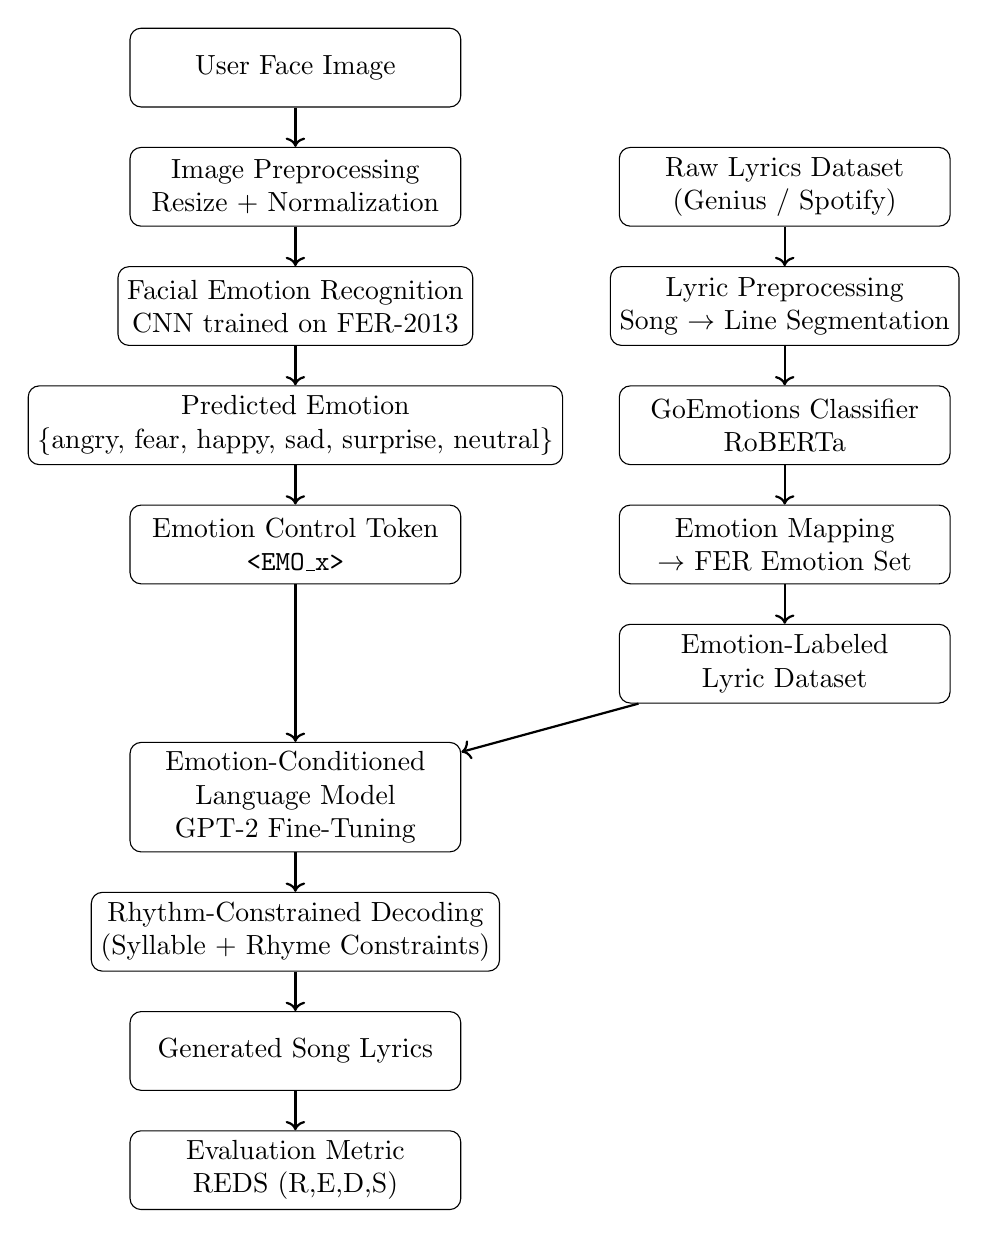
\begin{tikzpicture}[
node distance=0.5cm,
box/.style={draw, rectangle, rounded corners, align=center, minimum width=4.2cm, minimum height=1cm},
arrow/.style={->, thick}
]

% ---------- USER INPUT PIPELINE ----------

\node[box] (face)
{User Face Image};

\node[box, below=of face] (preprocess)
{Image Preprocessing\\
Resize + Normalization};

\node[box, below=of preprocess] (cnn)
{Facial Emotion Recognition\\
CNN trained on FER-2013};

\node[box, below=of cnn] (emotion)
{Predicted Emotion\\
$\{$angry, fear, happy, sad, surprise, neutral$\}$};

\node[box, below=of emotion] (token)
{Emotion Control Token\\
\texttt{<EMO\_x>}};

% ---------- DATASET PIPELINE ----------

\node[box, right=2cm of preprocess] (dataset)
{Raw Lyrics Dataset\\
(Genius / Spotify)};

\node[box, below=of dataset] (segment)
{Lyric Preprocessing\\
Song $\rightarrow$ Line Segmentation};

\node[box, below=of segment] (classifier)
{GoEmotions Classifier\\
RoBERTa};

\node[box, below=of classifier] (mapping)
{Emotion Mapping\\
$\rightarrow$ FER Emotion Set};

\node[box, below=of mapping] (labeled)
{Emotion-Labeled\\
Lyric Dataset};

% ---------- MODEL TRAINING ----------

\node[box, below=2cm of token] (gpt)
{Emotion-Conditioned\\
Language Model\\
GPT-2 Fine-Tuning};

\node[box, below=of gpt] (decoder)
{Rhythm-Constrained Decoding\\
(Syllable + Rhyme Constraints)};

\node[box, below=of decoder] (lyrics)
{Generated Song Lyrics};

\node[box, below=of lyrics] (eval)
{Evaluation Metric\\
REDS (R,E,D,S)};

% ---------- ARROWS ----------

\draw[arrow] (face) -- (preprocess);
\draw[arrow] (preprocess) -- (cnn);
\draw[arrow] (cnn) -- (emotion);
\draw[arrow] (emotion) -- (token);

\draw[arrow] (dataset) -- (segment);
\draw[arrow] (segment) -- (classifier);
\draw[arrow] (classifier) -- (mapping);
\draw[arrow] (mapping) -- (labeled);

\draw[arrow] (token) -- (gpt);
\draw[arrow] (labeled) -- (gpt);

\draw[arrow] (gpt) -- (decoder);
\draw[arrow] (decoder) -- (lyrics);
\draw[arrow] (lyrics) -- (eval);

\end{tikzpicture}

\end{document}